\documentclass[SKL-MASTER.tex]{subfiles}
\begin{document}
	\Large
\section*{Scaling data to the standard normal}
\begin{itemize}
\item A preprocessing step that is almost recommended is to scale columns to the standard
normal. 
\item The standard normal is probably the most important distribution of all statistics.
\item If you've ever been introduced to statistics, you must have almost certainly seen z-scores.
\item In truth, that's all this recipe is about—transforming our features from their endowed
distribution into z-scores.
\end{itemize}

\subsection*{Getting ready}
\begin{itemize}
\item The act of scaling data is extremely useful. There are a lot of machine learning algorithms,
which perform differently (and incorrectly) in the event the features exist at different scales.
\item For example, SVMs perform poorly if the data isn't scaled because it uses a distance function
in its optimization, which is biased if one feature varies from 0 to 10,000 and the other varies
from 0 to 1.
\end{itemize}
\newpage
The \textbf{preprocessing} module contains several useful functions to scale features. 	
Using the boston dataset, run the following commands:
%------------------------%
\begin{framed}
	\begin{verbatim}
	>>> from sklearn import preprocessing
	>>> import numpy as np # we'll need it later

	>>> X[:, :3].mean(axis=0) #mean of the first 3 features
	array([ 3.59376071, 11.36363636, 11.13677866])
	>>> X[:, :3].std(axis=0)
	array([ 8.58828355, 23.29939569, 6.85357058])
\end{verbatim}
\end{framed}
%------------------------ %
	There's actually a lot to learn from this initially. Firstly, the first feature has the smallest mean
	but varies even more than the third feature. The second feature has the largest mean and
	standard deviation—it takes the widest spread of values:
	%------------------------%
	\begin{framed}
		\begin{verbatim}
	>>> X_2 = preprocessing.scale(X[:, :3])
	>>> X_2.mean(axis=0)
	array([ 6.34099712e-17, -6.34319123e-16, -2.68291099e-15])
	>>> X_2.std(axis=0)
	array([ 1., 1., 1.])
\end{verbatim}
\end{framed}
%------------------------ %
	%===========================================================================================%
% %-	Premodel Workflow
% %	14
\newpage
\subsection*{Implementation} % %	How it works...
	The center and scaling function is extremely simple. It merely subtracts the mean and divides
	by the standard deviation:
\[ x_{scaled} = \frac{x-\bar{x}}{s} \]
%	In addition to a function, there is also a center and scaling class that is easy to invoke
%	and this is particularly useful when used in conjunction with the Pipelines mentioned later.
	It's also useful for the center and scaling class to persist across individual scaling:
	%------------------------%
	\begin{framed}
		\begin{verbatim}
	>>> my_scaler = preprocessing.StandardScaler()
	>>> my_scaler.fit(X[:, :3])
	>>> my_scaler.transform(X[:, :3]).mean(axis=0)
	array([ 6.34099712e-17, -6.34319123e-16, -2.68291099e-15])
\end{verbatim}
\end{framed}
%------------------------ %
\newpage
\subsection*{\texttt{MinMaxScaler}}
	Scaling features to mean 0, and standard deviation 1 isn't the only useful type of scaling.
	
	\begin{figure}[h!]
\centering
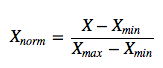
\includegraphics[width=0.5\linewidth]{minmax}
\end{figure}

	\textbf{\textit{Preprocessing}} also contains a \texttt{MinMaxScaler} class, which will scale the data within a
	certain range:
	%------------------------%
	\begin{framed}
	\begin{verbatim}
	>>> my_minmax_scaler = preprocessing.MinMaxScaler()
	>>> my_minmax_scaler.fit(X[:, :3])
	>>> my_minmax_scaler.transform(X[:, :3]).max(axis=0)
	array([ 1., 1., 1.])
	\end{verbatim}
\end{framed}
%------------------------ %
	It's very simple to change the minimum and maximum values of the \texttt{MinMaxScaler} class
	from its default of 0 and 1, respectively:
	%------------------------%
	
		\begin{verbatim}
	>>> Z_scaler = preprocessing.MinMaxScaler(feature_range=(-3,
	3))
	\end{verbatim}

%------------------------ %
\newpage
\subsection*{Normalization}
\textit{(N.B. Not related to Normal Distribution)}\\
	Furthermore, another option is \textbf{\textit{normalization}}. This will scale each sample to have a length of
	1. This is different from the other types of scaling done previously, where the features were
	scaled. 
	
Normalization is illustrated in the following command:
	%------------------------%
	\begin{framed}
		\begin{verbatim}
			>>> normalized_X = preprocessing.normalize(X[:, :3])
	\end{verbatim}
\end{framed}
%------------------------ %
\begin{itemize}
\item If it's not apparent why this is useful, consider the Euclidian distance (a measure of similarity)
	between three of the samples, where one sample has the values (1, 1, 0), another has (3, 3,
	0), and the final has (1, -1, 0).
\item	The distance between the 1st and 3rd vector is less than the distance between the 1st and 2nd
	though the 1st and 3rd are orthogonal, whereas the 1st and 2nd only differ by a scalar factor of
	3. 
\item Since distances are often used as measures of similarity, not normalizing the data first will
	be misleading
\end{itemize}


\section*{Creating binary features through thresholding}
\begin{itemize}
\item We  previously looked at transforming our data into the standard normal distribution.
\item Now, we'll talk about another transformation that is quite different.
%\item Instead of working with the distribution to standardize it, we'll purposely throw away data;
%but, if we have good reason, this can be a very smart move. 
\item Often, in what is ostensibly
continuous data, there are discontinuities that can be determined via binary features.
\end{itemize}

\subsection*{Getting ready}
Creating binary features and outcomes is a very useful method, but it should be used with
caution. Let's use the boston dataset to learn how to create turn values in binary outcomes.
First, load the boston dataset:
%------------------------%
\begin{framed}
\begin{verbatim}
>>> from sklearn import datasets
>>> boston = datasets.load_boston()
>>> import numpy as np
\end{verbatim}
\end{framed}
%------------------------ %
\subsection*{Implementation}
Similar to scaling, there are two ways to binarize features in scikit-learn:
\begin{enumerate}
\item \texttt{preprocessing.binarize }% #(a function)
\item \texttt{preprocessing.Binarizer} % #(a class)
\end{enumerate}

\subsection*{Boston Dataset}
The boston dataset's target variable is the median value of houses in thousands. This
dataset is good to test regression and other continuous predictors, but consider a situation
where we want to simply predict if a house's value is more than the overall mean. To do this,
we will want to create a threshold value of the mean. If the value is greater than the mean,
produce a 1; if it is less, produce a 0:
%--------------------------------------------- %
\begin{framed}
	\begin{verbatim}
>>> from sklearn import preprocessing
>>> new_target = preprocessing.binarize(boston.target,
threshold=boston.target.mean())
>>> new_target[:5]
array([ 1., 0., 1., 1., 1.])
\end{verbatim}
\end{framed}
%------------------------ %
This was easy, but let's check to make sure it worked correctly:
%--------------------------------------------- %
\begin{framed}
	\begin{verbatim}
>>> (boston.target[:5] > boston.target.mean()).astype(int)
array([1, 0, 1, 1, 1])
\end{verbatim}
\end{framed}
%------------------------ %
%===========================================================================================%
%-- Chapter 1
%-- Page 17

%Given the simplicity of the operation in NumPy, it's a fair question to ask why you will want
%to use the built-in functionality of scikit-learn. Pipelines, covered in the Using Pipelines
%for multiple preprocessing steps recipe, will go far to explain this; in anticipation of this,
%let's use the Binarizer class:
%--------------------------------------------- %
\begin{framed}
	\begin{verbatim}
>>> bin = preprocessing.Binarizer(boston.target.mean())
>>> new_target = bin.fit_transform(boston.target)
>>> new_target[:5]
array([ 1., 0., 1., 1., 1.])
\end{verbatim}
\end{framed}
%---------------------------------------------- %
% How it works...
% Hopefully, this is pretty obvious; but under the hood, scikit-learn creates a conditional mask
% that is True if the value in the array in question is more than the threshold. It then updates
% the array to 1 where the condition is met, and 0 where it is not.
% There's more...
% Let's also learn about sparse matrices and the fit method.
\subsection*{Sparse matrices}
Sparse matrices are special in that zeros aren't stored; this is done in an effort to save space
in memory. This creates an issue for the binarizer, so to combat it, a special condition for the
binarizer for sparse matrices is that the threshold cannot be less than zero:
%--------------------------------------------- %
\begin{framed}
	\begin{verbatim}
>>> from scipy.sparse import coo
>>> spar = coo.coo_matrix(np.random.binomial(1, .25, 100))
>>> preprocessing.binarize(spar, threshold=-1)

ValueError: Cannot binarize a sparse matrix with threshold < 0
\end{verbatim}
\end{framed}
%---------------------------------------------- %
%\subsection*{The fit method}
%The fit method exists for the binarizer transformation, but it will not fit anything, it will simply
%return the object.

\newpage
\section*{Working with categorical variables}
\begin{itemize}
\item Categorical variables are a problem. On one hand they provide valuable information; on the
other hand, it's probably text—either the actual text or integers corresponding to the text—like
an index in a lookup table.
\item So, we clearly need to represent our text as integers for the model's sake, but we can't just use
the id field or naively represent them. 
\item This is because we need to avoid a similar problem to the
\item Creating binary features through thresholding recipe. If we treat data that is continuous, it must
be interpreted as continuous.
\end{itemize}
%===========================================================================================%
%-- Premodel Workflow
%-- 18
\subsubsection*{Getting ready}
\begin{itemize}
\item 
The boston dataset won't be useful for this section. While it's useful for feature binarization,
it won't suffice for creating features from categorical variables.
\item For this, the iris dataset
will suffice.
For this to work, the problem needs to be turned on its head. 
\item Imagine a problem where the
goal is to predict the sepal width; therefore, the species of the flower will probably be useful
as a feature.
\end{itemize}
Let's get the data sorted first:

%------------------------%
\begin{framed}
\begin{verbatim}
>>> from sklearn import datasets
>>> iris = datasets.load_iris()
>>> X = iris.data
>>> y = iris.target
\end{verbatim}
\end{framed}
%---------------------------------------------- %
Now, with X and Y being as they normally will be, we'll operate on the data as one:
%------------------------%
\begin{framed}
\begin{verbatim}
>>> import numpy as np
>>> d = np.column_stack((X, y))
\end{verbatim}
\end{framed}
%---------------------------------------------- %
\subsection*{Implementation}
Convert the text columns to three features:
%--------------------------------------------- %
\begin{framed}
\begin{verbatim}
>>> from sklearn import preprocessing
>>> text_encoder = preprocessing.OneHotEncoder()
>>> text_encoder.fit_transform(d[:, -1:]).toarray()[:5]
array([[ 1., 0., 0.],
[ 1., 0., 0.],
[ 1., 0., 0.],
[ 1., 0., 0.],
[ 1., 0., 0.]])
\end{verbatim}
\end{framed}
%---------------------------------------------- %
\subsection*{Implementation}
\begin{itemize}
\item The encoder creates additional features for each categorical variable, and the value returned
is a sparse matrix. 
\item The result is a sparse matrix by definition; each row of the new features has
0 everywhere, except for the column whose value is associated with the feature's category.
\item Therefore, it makes sense to store this data in a sparse matrix.
\texttt{text\_encoder} is now a standard scikit-learn model, which means that it can be used again:
\end{itemize}

\begin{framed}
\begin{verbatim}
>>> text_encoder.transform(np.ones((3, 1))).toarray()
array([[ 0., 1., 0.],
[ 0., 1., 0.],
[ 0., 1., 0.]])
\end{verbatim}
\end{framed}
%===========================================================================================%
%-- Chapter 1
% % -19
\subsubsection*{DictVectorizer}
Another option is to use DictVectorizer. This can be used to directly convert strings
to features:
%------------------------%
\begin{framed}
\begin{verbatim}
>>> from sklearn.feature_extraction import DictVectorizer
>>> dv = DictVectorizer()
>>> my_dict = [{'species': iris.target_names[i]} for i in y]
>>> dv.fit_transform(my_dict).toarray()[:5]
array([[ 1., 0., 0.],
[ 1., 0., 0.],
[ 1., 0., 0.],
[ 1., 0., 0.],
[ 1., 0., 0.]])
\end{verbatim}
\end{framed}
Dictionaries can be viewed as a sparse matrix. They only contain
entries for the nonzero values.

\newpage
\section*{Binarizing label features}
Now we'll look at working with categorical variables in a different way. In the event
that only one or two categories of the feature are important, it might be wise to avoid the
extra dimensionality, which might be created if there are several categories.
\subsubsection*{Getting ready}
\begin{itemize}
\item There's another way to work with categorical variables.
\item Instead of dealing with the categorical
variables using \texttt{OneHotEncoder}, we can use \texttt{LabelBinarizer}. 
\item This is a combination of
thresholding and working with categorical variables.
\end{itemize}

To show how this works, load the iris dataset:
\begin{framed}
\begin{verbatim}
>>> from sklearn import datasets as d
>>> iris = d.load_iris()
>>> target = iris.target
\end{verbatim}
\end{framed}
%================================================================================================= %
\subsubsection*{Implementation}
Import the \texttt{LabelBinarizer()} method and create an object. Then transform the target outcomes to the new feature space.
\begin{framed}
\begin{verbatim}

>>> from sklearn.preprocessing import LabelBinarizer
>>> label_binarizer = LabelBinarizer()

>>> new_target = label_binarizer.fit_transform(target)
\end{verbatim}
\end{framed}
Let's look at \texttt{new\_target} and the \texttt{label\_binarizer} object to get a feel of what happened:

%===========================================================================================%
%-- Chapter 1
21
\begin{framed}
\begin{verbatim}
>>> new_target.shape
(150, 3)
>>> new_target[:5]
array([[1, 0, 0],
[1, 0, 0],
[1, 0, 0],
[1, 0, 0],
[1, 0, 0]])
>>>
>>> new_target[-5:]
array([[0, 0, 1],
[0, 0, 1],
[0, 0, 1],
[0, 0, 1],
[0, 0, 1]])
>>>
>>> label_binarizer.classes_
array([0, 1, 2])
\end{verbatim}
\end{framed}
\subsubsection*{Theoretical Matters}
The iris target has a cardinality of 3, that is, it has three unique values. When
\texttt{LabelBinarizer} converts the vector N x 1 into the vector N x C, where C is the
cardinality of the N x 1 dataset, it is important to note that once the object has been
fit, introducing unseen values in the transformation will throw an error:
\begin{framed}
\begin{verbatim}
>>> label_binarizer.transform([4])
[...]
ValueError: classes [0 1 2] mismatch with the labels [4] found in the
data
\end{verbatim}
\end{framed}
\subsection*{Other Remarks}
\begin{itemize}
\item Zero and one do not have to represent the positive and negative instances of the target
value. 
\item For example, if we want positive values to be represented by 1,000, and negative
values to be represented by -1,000, we'd simply make the designation when we create
\texttt{label\_binarizer}:
\end{itemize}

%------------------------%
\begin{framed}
\begin{verbatim} 
>>> label_binarizer = LabelBinarizer(neg_label=-1000,
pos_label=1000)
>>> label_binarizer.fit_transform(target)[:5]
array([[ 1000, -1000, -1000],
[ 1000, -1000, -1000],
[ 1000, -1000, -1000],
[ 1000, -1000, -1000],
[ 1000, -1000, -1000]])
\end{verbatim}
\end{framed}
The only restriction on the positive and negative values
is that they must be integers.
\end{document}


	%===========================================================================================%
	%-- Chapter 1
	%	15
	..
	%	There's more...
	%	Imputation is a very deep subject. Here are a few things to consider when using
	%	scikit-learn's implementation.
	\section*{Creating idempotent scalar objects}
	\begin{itemize}
		\item It is possible to scale the mean and/or variance in the \texttt{StandardScaler} instance.
		\item For instance, it's possible (though not useful) to create a \texttt{StandardScaler} instance,
		which simply performs the identity transformation:
	\end{itemize}
	
	%------------------------%
	\begin{framed}
		\begin{verbatim}
		>>> my_useless_scaler = preprocessing.StandardScaler(with_mean=False,
		with_std=False)
		>>> transformed_sd = my_useless_scaler
		.fit_transform(X[:, :3]).std(axis=0)
		>>> original_sd = X[:, :3].std(axis=0)
		>>> np.array_equal(transformed_sd, original_sd)
		\end{verbatim}
	\end{framed}
	%------------------------ %
	%======================================================== %
	\subsection*{Handling sparse imputations}
	Sparse matrices aren't handled differently from normal matrices when doing scaling. This is
	because to mean center the data, the data will have its 0s altered to nonzero values, thus the
	matrix will no longer be sparse:
	%------------------------%
	\begin{framed}
		\begin{verbatim}
		>>> matrix = scipy.sparse.eye(1000)
		>>> preprocessing.scale(matrix)
		…
		ValueError: Cannot center sparse matrices: pass 'with_mean=False' instead
		See docstring for motivation and alternatives.
		
		As noted in the error, it is possible to scale a sparse matrix with_std only:
		>>> preprocessing.scale(matrix, with_mean=False)
		<1000x1000 sparse matrix of type '<type 'numpy.float64'>'
		with 1000 stored elements in Compressed Sparse Row format>
		The other option is to call todense() on the array. However, this is dangerous because the
		matrix is already sparse for a reason, and it will potentially cause a memory error.
		\end{verbatim}
	\end{framed}	
	%===========================================================================================%
	% % Premodel Workflow
	% % 16
	
	\newpage
	\subsection*{Patsy}
	\begin{itemize}
		\item patsy is another package useful to encode categorical variables. 
		\item Often used in conjunction
		with \textbf{\textit{StatsModels}}, patsy can turn an array of strings into a design matrix.
		\item This section does not directly pertain to scikit-learn; therefore,
		skipping it is okay without impacting the understanding of how
		scikit-learn works.
		\item For example, \texttt{dm = patsy.design\_matrix("x + y")} will create the appropriate
		columns if x or y are strings. 
		\item If they aren't, C(x) inside the formula will signify that it
		is a categorical variable.
		\item For example, iris.target can be interpreted as a continuous variable if we don't know
		better. 
	\end{itemize}
	Therefore, use the following command:
	
	%===========================================================================================%
	% % Premodel Workflow
	% % 20
	\begin{framed}
		\begin{verbatim}
		>>> import patsy
		>>> patsy.dmatrix("0 + C(species)", {'species': iris.target})
		DesignMatrix with shape (150, 3)
		
		C(species)[0] C(species)[1] C(species)[2]
		1 0 0
		1 0 0
		1 0 0
		1 0 0
		1 0 0
		1 0 0
		1 0 0
		1 0 0
		1 0 0
		[...]
		\end{verbatim}
	\end{framed}
	
\subsubsection*{Other Remarks}
Other options exist to create categorical variables in scikit-learn and Python at large.
\texttt{DictVectorizer} is a good option if you like to limit the dependencies of your projects
to only scikit-learn and you have a fairly simple encoding scheme. However, if you require
more sophisticated categorical encoding, patsy is a very good option.
